

\chapter[Introduction to Image Processing and the MATLAB Environment]{Introduction to Image Processing and the\\ MATLAB Environment}


\chapterinitial{A}{COMPONENT PART} for an electronic item is
manufactured at one of three different factories, and then delivered to
the main assembly line.Of the total number supplied, factory A supplies
50\%, factory B 30\%, and factory C 20\%. Of the components
manufactured at factory A, 1\% are faulty and the corresponding
proportions for factories B and C are 4\% and 2\% respectively. A
component is picked at random from the assembly line. 


\section{Introduction}\label{intro}
The term reliability usually refers to the probability that a
component or system will operate satisfactorily either at any particular
instant at which it is required or for a certain length of
time. Fundamental to quantifying reliability s a knowledge of how to
define, assess and combine probabilities \cite{Bontempi2005Adaptive}. This may hinge on identifying the
form of the variability which is nherent n most processes. If all
components had a fixed known lifetime there would be no need to model
reliability.


\subsection{A Comp\'onent Part}
A component part for an electronic item is
manufactured at one of three different factories, and then delivered to
the main assembly line.Of the total number supplied, factory A supplies
50\%, factory B 30\%, and factory C 20\%. Of the components
manufactured at factory A, 1\% are faulty and the corresponding
proportions for factories B and C are 4\% and 2\% respectively. A
component is picked at random from the assembly line. What is the
probability that it is faulty \cite{ilyas2004hsn}? 
A component part for an electronic item is
manufactured at one of three different factories, and then delivered to
the main assembly line. Of the total number supplied, factory A supplies
50\%, factory B 30\%, and factory C 20\%. Of the components
manufactured at factory A, 1\% are faulty and the corresponding
proportions for factories B and C are 4\% and 2\% respectively. A
component is picked at random from the assembly line. What is the
probability that it is faulty? 
A component part for an electronic item is
manufactured at one of three different factories, and then delivered to
the main assembly line.Of the total number supplied, factory A supplies
50\%, factory B 30\%, and factory C 20\%. Of the components
manufactured at factory A, 1\% are faulty and the corresponding
proportions for factories B and C are 4\% and 2\% respectively. A
component is picked at random from the assembly line. What is the
probability that it is faulty? 

A component part for an electronic item is
manufactured at one of three different factories, and then delivered to
the main assembly line.Of the total number supplied, factory A supplies
50\%, factory B 30\%, and factory C 20\%. Of the components
manufactured at factory A, 1\% are faulty and the corresponding
proportions for factories B and C are 4\% and 2\% respectively. A
component is picked at random from the assembly line. What is the
probability that it is faulty \cite{ilyas2004hsn}? 
A component part for an electronic item is
manufactured at one of three different factories, and then delivered to
the main assembly line.Of the total number supplied, factory A supplies
50\%, factory B 30\%, and factory C 20\%. Of the components
manufactured at factory A, 1\% are faulty and the corresponding
proportions for factories B and C are 4\% and 2\% respectively. A
component is picked at random from the assembly line. What is the
probability that it is faulty? 
A component part for an electronic item is
manufactured at one of three different factories, and then delivered to
the main assembly line.Of the total number supplied, factory A supplies
50\%, factory B 30\%, and factory C 20\%. Of the components
manufactured at factory A, 1\% are faulty and the corresponding
proportions for factories B and C are 4\% and 2\% respectively. A
component is picked at random from the assembly line. What is the
probability that it is faulty? 

\begin{table}%1
\tabcolsep6pt
%\noautomaticrules
\tabletitle{Comparison of C and MATLAB Code for Simple Matrix Operations}%
\begin{tabular}{@{}lccc@{}}
\tch{Operations}    &\tch{Part of C Code} &\tch{Hor. fts.} &\tch{Ver. fts.}\\[-2pt]
Ball &19, 221 &4, 598   &3, 200\\
Pepsi$^a$&46, 281 &6, 898 &5, 400\\
Keybrd$^b$   &27, 290 &2, 968 &3, 405\\
Pepsi    &14, 796 &9, 188 &3, 209\\
\end{tabular}
\end{table}

A components part for an electronic item is
manufactured at one of three different factories, and then delivered to
the main assembly line.Of the total number supplied, factory A supplies
50\%, factory B 30\%, and factory C 20\%. Of the components
manufactured at factory A, 1\% are faulty and the corresponding
proportions for factories B and C are 4\% and 2\% respectively. A
component is picked at random from the assembly line. What is the
probability that it is faulty \cite{ilyas2004hsn}? 
A component part for an electronic item is
manufactured at one of three different factories, and then delivered to
the main assembly line.Of the total number supplied, factory A supplies
50\%, factory B 30\%, and factory C 20\%. Of the components
manufactured at factory A, 1\% are faulty and the corresponding
proportions for factories B and C are 4\% and 2\% respectively. A
component is picked at random from the assembly line. What is the
probability that it is faulty? 
A component part for an electronic item is
manufactured at one of three different factories, and then delivered to
the main assembly line.Of the total number supplied, factory A supplies
50\%, factory B 30\%, and factory C 20\%. Of the components
manufactured at factory A, 1\% are faulty and the corresponding
proportions for factories B and C are 4\% and 2\% respectively. A
component is picked at random from the assembly line. What is the
probability that it is faulty? 



\begin{VF}
``A Process is a structured, measured set of activities designed to produce a specific output for a particular customer
or market---A process is thus a specific ordering of work activities across time and space, with a beginning, an end.
and clearly defined inputs and outputs: a structure for action.''

\VA{Thomas Davenport}{Senior Adjutant to the Junior Marketing VP}
\end{VF}


\begin{table}%1
\tabcolsep8pt
%\noautomaticrules
\tabletitle{Comparison of MATLAB and C Code for Simple Matrix Operations}%
\begin{tabular}{@{}lccc@{}}
\tch{Operations}    &\tch{Part of C Code} &\tch{Hor. fts.} &\tch{Ver. fts.}\\[-2pt]
Ball &19, 221 &4, 598   &3, 200\\
Pepsi$^a$&46, 281 &6, 898 &5, 400\\
Keybrd$^b$   &27, 290 &2, 968 &3, 405\\
Pepsi    &14, 796 &9, 188 &3, 209\\
\end{tabular}
\end{table}

\textbf{MultiRelational $k$-Anonymity.} Most works on $k$-anonymity focus on anonymizing a single data table; however, a real-life \cite{diamantaras1996pcn} database usually contains multiple relational tables. This has proposed a privacy model called \emph{MultiR $k$-anonymity} to ensure $k$-anonymity on multiple relational tables. Their model assumes that a relational database contains a person-specific table $PT$ and a set of tables $T_1,\cdots,T_n$, where $PT$ contains a person identifier $Pid$ and some sensitive attributes, and $T_i$, for $1 \leq i \leq n$, contains some foreign keys, some attributes in $QID$, and sensitive attributes. The general privacy notion is to ensure that for each record owner $o$ contained in the join of all tables $PT \Join T_1 \Join \cdots \Join T_n$, there exists at least $k-1$ other record owners share the same $QID$ with $o$. It is important to emphasize that the $k$-anonymization is applied at the \emph{record owner} level, not at the \emph{record} level in traditional $k$-anonymity. This idea is similar to $(X,Y)$-anonymity, where $X=QID$ and $Y=\{Pid\}$.

\begin{table}[b!]%2
\tabcolsep10pt
\tabletitle{Now we are engaged $(a_g^a)$ $\big(a_g^a\big)$ in a great civil war, testing whether that
nation, or any nation so conceived.}%}{%[Short Table Caption]
\begin{tabular}{@{}lccc@{}}
%%\tch{Scene}    &\tch{Reg. fts.} &\tch{Hor. fts.} &\tch{Ver. fts.}\\
%%\multicolumn{4}{@{}l@{}}{\tsh{Table Head}}\\[3pt]\hline\\[-6pt]
Ball &19, 221 &4, 598   &3, 200\\
Pepsi &46, 281 &6, 898 &5, 400\\
Keybrd   &27, 290 &2, 968 &3, 405\\
Pepsi    &14, 796 &9, 188 &3, 209\\
\end{tabular}
\end{table}

%%\begin{shadebox}
%%A component part for an electronic item is
%%manufactured at one of three different factories, and then delivered to
%%the main assembly line.Of the total number supplied, factory A supplies
%%50\%, factory B 30\%, and factory C 20\%. Of the components
%%manufactured at factory A, 1\% are faulty and the corresponding
%%proportions for factories B and C are 4\% and 2\% respectively. A
%%component is picked at random from the assembly line. What is the
%%probability that it is faulty? 
%%\end{shadebox}

\begin{enumerate}
\item Factual knowledge (``knowing that") One family considers a privacy
threat occurs when an attacker is able to link a record owner to a record
in a published data table, to a sensitive attribute in a published data
table, or to the published data table itself. We call them \emph{record
linkage}, \emph{attribute linkage}.
\begin{enumerate}
\item Conceptual knowledge (``knowing why") One family considers a privacy
threat occurs when an attacker is able to link a record owner to a record
in a published data table, to a sensitive attribute in a published data
table, or to the published data table itself. We call them \emph{record
linkage}, \emph{attribute linkage}.
\begin{enumerate}
\item Procedual knowledge (``knowing what") One family considers a privacy
threat occurs when an attacker is able to link a record owner to a record
in a published data table, to a sensitive attribute in a published data
table, or to the published data table itself. We call them \emph{record
linkage}, \emph{attribute linkage}.
\item Spatial knowledge (``knowing what")
\end{enumerate}
\end{enumerate}
\end{enumerate}

In most literature on PPDP, they \cite{jolliffe2002pca} consider a more relaxed, yet more practical, notion of privacy protection by assuming limited attacker's background knowledge. Below, the term ``victim" refers to the record owner being linked. We can broadly classify linking models to two families.

\begin{extract}
A component part for an electronic item is \cite{hyvarinen2001ica}
manufactured at one of three different factories, and then delivered to
the main assembly line.Of the total number supplied, factory A supplies
50\%, factory B 30\%, and factory C 20\%. Of the components
manufactured at factory A, 1\% are faulty and the corresponding
proportions for factories B and C are 4\% and 2\% respectively. 
\end{extract}

In most literature on PPDP, they \cite{jolliffe2002pca} consider a more relaxed, yet more practical, notion of privacy protection by assuming limited attacker's background knowledge. Below, the term ``victim" refers to the record owner being linked. We can broadly classify linking models to two families.

\begin{itemize}
\item Factual knowledge (``knowing that") One family considers a privacy
threat occurs when an attacker is able to link a record owner to a record
in a published data table, to a sensitive attribute in a published data
table, or to the published data table itself. We call them \emph{record
linkage}, \emph{attribute linkage}.
\begin{itemize}
\item Conceptual knowledge (``knowing why") One family considers a privacy
threat occurs when an attacker is able to link a record owner to a record
in a published data table, to a sensitive attribute in a published data
table, or to the published data table itself. We call them \emph{record
linkage}, \emph{attribute linkage}.
\begin{itemize}
\item Procedual knowledge (``knowing what") One family considers a privacy
threat occurs when an attacker is able to link a record owner to a record
in a published data table, to a sensitive attribute in a published data
table, or to the published data table itself. We call them \emph{record
linkage}, \emph{attribute linkage}.
\item Spatial knowledge (``knowing what")
\end{itemize}
\end{itemize}
\end{itemize}


One family considers a privacy threat occurs when an attacker is able to link a record owner to a record in a published data table, to a sensitive attribute in a published data table, or to the published data table itself. We call them \emph{record linkage}, \emph{attribute linkage}, and \emph{table linkage}, respectively. In all types of linkages, we assume that the attacker knows the $QID$ of the victim. In record and attribute linkages, we further assume that the attacker knows the presence of the victim's record in the released table, and seeks to identify the victim's record and/or sensitive information from the table \cite{yao2002can}. In table linkage, the attack seeks to determine the present or absent of the victim's record in the released table. A data table is considered to privacy preserved if the table can effectively prevent the attacker from successfully performing these types of linkages on the table \cite{madden2002tta}. Sections~\ref{intro}-\ref{sec:reclinkage} study this family of privacy models.
\begin{equation}
\mbox{var}\widehat{\Delta} = \sum_{j = 1}^t \sum_{k = j+1}^t
\mbox{var}\,(\hat{\alpha}_j - \hat{\alpha}_k)  = \sum_{j = 1}^t
\sum_{k = j+1}^t \sigma^2(1/n_j + 1/n_k). \label{2delvart2}
\end{equation}


An obvious measure of imbalance is just the difference in the
number of times the two treatments are allocated
\begin{equation}
D_n = \mathcal{M}|n_A - n_B|. \label{2deffD}
\end{equation}
For rules such as deterministic allocation, for which the expected
value of this difference can be calculated, we obtain the population
value ${\cal D}_n$.

%%\begin{shortbox}
%%\Boxhead{Box Title Here}
%%Another family aims at achieving the \emph{uninformative principle}: The published table should provide the attacker with little additional information beyond the background knowledge. There should not be a large difference between the prior and posterior beliefs; otherwise, there is a privacy threat~\cite{jain2004ass, jolliffe2002pca}. Many privacy models in this family are designed for statistical database and do not distinguish attributes in $T$ into $QID$, but some of them could also thwart record, attribute, and table linkages. Section~\ref{intro} studies this family of privacy models.
%%
%%Let $m$ be a prime number. With the addition and multiplication as 
%%defined above, $Z_m$ is a field.
%%\end{shortbox}

\begin{theorem}\label{1th:Z_m}
Let $m$ be a prime number. With the addition and multiplication as 
defined above, $Z_m$ is a field.
\end{theorem}

\begin{proof}
Most of the proof of this theorem is routine.  It is clear that $0\in Z_m$ 
and $1\in Z_m$ are the 
zero element and identity element. If $a\in Z_m$ and $a\ne 0$, then $m-a$ 
is the additive inverse of $a$. If $a\in Z_m$ and $a\ne 0$, then the 
greatest common divisor of $a$ and $m$ is 1, and hence
there exist integers $s$ and $t$ such that $sa+tm=1$. Thus $sa=1 -tm$ is 
congruent to 1 modulo $m$. Let $s^*$ be the integer in $Z_m$ 
congruent to $s$ 
modulo $m$. Then we also have $s^*a\equiv 1\  \mbox{mod}\ m$. Hence $s^*$ 
is 
the multiplicative inverse of $a$ modulo $m$. Verification of the rest of 
the field properties is now routine.\end{proof}



\section{Record Linkage Model}\label{sec:reclinkage}

In the privacy attack of \emph{record linkage}, some value $qid$ on $QID$ identifies a small number of records in the released table $T$,
called a \emph{group}. If the victim's $QID$ matches the value
$qid$, the victim is vulnerable to being linked to the small
number of records in the group \cite{madden2005taq}. In this case, the attacker faces
only a small number of possibilities for the victim's record, and
with the help of additional knowledge, there is a chance that the
attacker could uniquely identify the victim's record from the
group.


%%%\begin{table}
%%%    \tabletitle{Examples for illustrating attacks}
%%%    \begin{tabular}{|c|c|c|c|}
%%%        \hline
%%%        \textbf{Job} & \textbf{Sex} & \textbf{Age} & \textbf{Disease} \\
%%%        \hline
%%%        Engineer & Male & 35 & Hepatitis \\
%%%        Engineer & Male & 38 & Hepatitis \\
%%%        Lawyer & Male & 38 & HIV \\
%%%        Writer & Female & 30 & Flu \\
%%%        Writer & Female & 30 & HIV \\
%%%        Dancer & Female & 30 & HIV \\
%%%        Dancer & Female & 30 & HIV \\
%%%        \hline
%%%    \end{tabular}
%%%    \label{table:rawpatient}
%%%\end{table}



\subsection{A Component Part}
A component part for an electronic item is
manufactured at one of three different factories, and then delivered to
the main assembly line.Of the total number supplied, factory A supplies
50\%, factory B 30\%, and factory C 20\%. Of the components
manufactured at factory A, 1\% are faulty and the corresponding
proportions for factories B and C are 4\% and 2\% respectively. A
component is picked at random from the assembly line. What is the
probability that it is faulty? 



\begin{figure}\centering
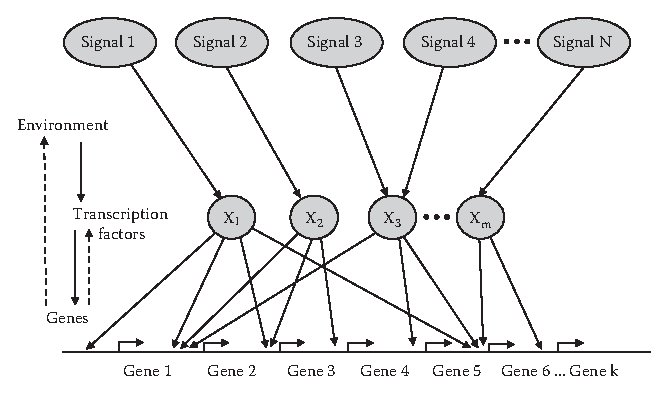
\includegraphics{Chapters/chapter1/figures/002x001.eps}
\caption[List of figure caption goes here]{Figure caption goes here.}
\end{figure}



\begin{figure}[htb]
\centering
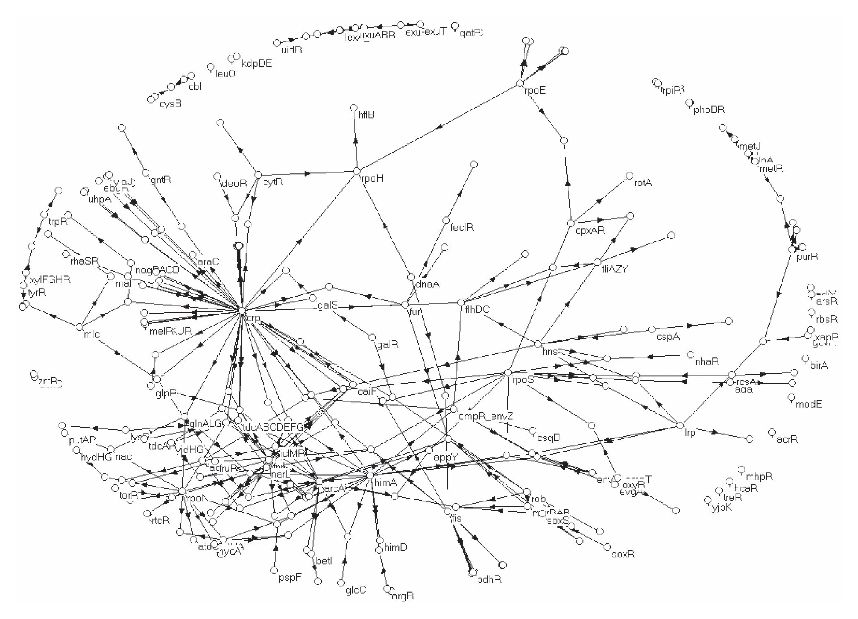
\includegraphics[width=\textwidth]{Chapters/chapter1/figures/002x003.eps}
\caption[Short figure caption]{Figure caption goes here. Figure caption goes here.
Figure caption goes here. Figure caption goes here. Figure caption goes here.
Figure caption goes here.}
\end{figure}






\subsubsection{H3 A Component Part }
A component part for an electronic item is
manufactured at one of three \cite{mardia1979ma} different factories, and then delivered to
the main assembly line.Of the total number supplied, factory A supplies
50\%, factory B 30\%, and factory C 20\%. Of the components
manufactured at factory A, 1\% are faulty and the corresponding
proportions for factories B and C are 4\% and 2\% respectively. A
component is picked at random from the assembly line. What is the
probability that it is faulty? 

\paragraph{H4 A Component Part }
A fundamental notion \cite{yao2002can} is that of a\index{subspace}\index{vector 
space!subspace of} subspace of $F^n$. Let $V$ be a nonempty subset of 
$F^n$. Then $V$ is a {\it subspace} of $F^n$ provided $V$ is closed 
under vector addition and scalar multiplication, that is, 

\subparagraph{H5 A Component Part }
A fundamental notion \cite{yao2002can} is that of a\index{subspace}\index{vector 
space!subspace of} subspace of $F^n$. Let $V$ be a nonempty subset of 
$F^n$. Then $V$ is a {\it subspace} of $F^n$ provided $V$ is closed 
under vector addition and scalar multiplication, that is, 
\begin{enumerate}
\item For all $u$ and $v$ in $V$, $u+v$ is 
also in $V$. 
\item For all $u$ in $V$ and $c$ in $F$, $cu$ is 
in $V$. 
\end{enumerate} 
Let $u$ be in the subspace $V$. Because $0u=0$, 
it follows that the zero vector is in $V$. Similarly, $-u$ is in $V$ 
for all $u$ in $V$. A simple example of a subspace of $F^n$ is the set 
of all vectors $(0,a_2,\ldots,a_n)$ with first coordinate equal to 0. 
The zero vector itself is a subspace.

\begin{definition}\label{1def:linearcomb}{\rm
Let $u^{(1)},u^{(2)},\ldots,u^{(m)}$ be vectors in $F^n$, and let 
$c_1,c_2,\ldots,c_m$ be scalars. Then the vector
\[c_1u^{(1)}+c_2u^{(2)}+\cdots+c_mu^{(m)}\]
is called a {\it linear combination} \index{linear combination} of $u^{(1)},u^{(2)},\ldots,u^{(m)}$.
If $V$ is a subspace of $F^n$, then $V$ is closed under vector addition and 
scalar multiplication, and it follows easily by induction that a 
linear combination of vectors in $V$ is also a vector in $V$. Thus 
{\it subspaces 
are closed under linear combinations}; in fact, this can be taken as the 
defining property of subspaces.
The vectors $u^{(1)},u^{(2)},\ldots,u^{(m)}$ {\it span} $V$ \index{spanning set}
(equivalently, form a {\it spanning set} of $V$) provided every vector in 
$V$ 
is a linear combination of $u^{(1)},u^{(2)},\ldots,u^{(m)}$. The zero 
vector can be written as a linear combination of 
$u^{(1)},u^{(2)},\ldots,u^{(m)}$ with all scalars equal to 0; this is a 
{\it trivial linear combination}.\index{linear combination!trivial} The vectors
$u^{(1)},u^{(2)},\ldots,u^{(m)}$ are {\it linearly dependent} provided 
there are scalars $c_1,c_2,\ldots,c_m$, not all of which are zero, such 
that
\[c_1u^{(1)}+c_2u^{(2)}+\cdots+c_mu^{(m)}=0,\]
that is, the zero vector can be written as a {\it nontrivial linear \index{linear combination!nontrivial} 
combination}\break of $u^{(1)},u^{(2)},\ldots,u^{(m)}$.
For example, the vectors $(1,4), (3,-1)$, and $(3,5)$ in $\Re^2$ are 
linearly 
dependent since
\[3(1,4)+1(3,-2)-2(3,5)=(0,0).\] Vectors are {\it linearly independent} provided  they are not linearly dependent.\index{linearly independent}
The vectors 
$u^{(1)},u^{(2)},\ldots,u^{(m)}$ are a {\it basis} \index{basis} of $V$ provided they are  
linearly independent and span $V$.
By an {\it ordered basis} \index{basis!ordered} we mean a basis in which the vectors of the basis are listed 
in a specified order; to indicate that we have an ordered basis we write
$(u^{(1)},u^{(2)},\ldots,u^{(m)})$. 
A spanning set $S$ of $V$ is a \index{spanning set!minimal} {\it minimal spanning set of $V$} provided that
each set 
of vectors obtained from $S$ by removing a vector is not a spanning set 
for $V$.
A linearly independent set $S$ of vectors of $V$ is a {\it maximal linearly \index{linearly independent!maximal}
independent set of vectors of $V$} provided that for each vector $w$ of 
$V$ that 
is not in $S$, $S\cup\{w\}$ is  linearly dependent (when this happens, 
$w$ must be  a linear combination of the vectors in 
$S$).\hfill{$\Box$}
}\end{definition}

In addition to matrix addition, subtraction, and multiplication, there is 
one additional operation that we define now. It's perhaps the simplest of 
them all. Let $A=[a_{ij}]$ be an $m$ by $n$ matrix and let $c$ be a 
number \cite{hyvarinen2001ica}. Then the matrix $c\cdot A$, or simply $cA$, is the $m$ by $n$ 
matrix obtained by multiplying each entry of $A$ by $c$:
\[c A=[ca_{ij}].\]\index{matrix!scalar multiplication} \index{matrix!scalar multiple of}
The matrix $c A$ is called a {\it scalar multiple} of $A$.

\begin{verbatim}
<spec>        ::= <module> {<module>}   

<module>      ::= <fun> |  <init> | <host> | <channel> |

<fun>         ::= "fun" <funname> { ";" "fun" <funname> }

<funname>     ::= <name> <funpar> 

<funpar>      ::= [ "(" <name> { "," <name> } ")" ] 
                      [ "[" <qop> { ";" <qop>} "]" ]
\end{verbatim}

In addition to matrix addition, subtraction, and multiplication, there is 
one additional operation that we define now. It's perhaps the simplest of 
them all. Let $A=[a_{ij}]$ be an $m$ by $n$ matrix and let $c$ be a 
number \cite{hyvarinen2001ica}. Then the matrix $c\cdot A$, or simply $cA$, is the $m$ by $n$ 
matrix obtained by multiplying each entry of $A$ by $c$:
\[c A=[ca_{ij}].\]\index{matrix!scalar multiplication} \index{matrix!scalar multiple of}
The matrix $c A$ is called a {\it scalar multiple} of $A$.

\begin{verbatim}

<letter>      ::= "a" | "b" | "c" | "d" | "e" | "f" | "g" | 
                  "h" | "i" | "j" | "k" | "l" | "m" | "n" |
                  "o" | "p" | "q" | "r" | "s" |
                  "v" | "w" | "x" | "y" | "z" | "A" | "B" |
                   "C" | "D" | "E" | "F" | "G" |
                  "J" | "K" | "L" | "M" | "N" | "O" | "P" |
                   "Q" | "R" | "S" | "T"|  "U" |
                  "X" | "Y" | "Z" |"_"

<digit>       ::= "0" | "1" | "2" | "3" | "4" | "5" | "6" |
                     "7" | "8" | "9"

<value>       ::= <digit> { <digit> } [ "." { <digit> } ]

<init>        ::= "init" "{" "version" <value> { "," <value> } "}" 

<version>     ::= "version" <value> "{" <run> "}"
                  { "version" <value> "{" <run> "}"}

<run>         ::= "run" <name> <par> [ <rep> ] [ <chrep> ]| 
                  "run" <name> <par> [ <rep> ] [ <chrep> ]
                  "->" "run" <name> <par> [ <rep> ] [ <chrep> ]

<par>         ::= "(" [ <name> { "," <name> } | "*" ] ")"
		
<rep>         ::= "{" <valuei> "}"

<chrep>       ::= "[" <name> "." <valuei> 
                        { "," <name> "." <valuei> } "]"
		
<host>        ::= "host" <hostpar> { "host" <hostpar> }

<hostpar>     ::= <name> "(" <sche> ")" "(" <hchan> ")"
                       "{" <hbody> "}"

<sche>        ::=  "fifo" | "rr"

<hchan>       ::= <name> | "*" 

<hbody>       ::= <process> | <#>

<process>     ::= "process" <name> <par> "{" <procpar> "}" 
                  { "process" <name> <par>
                   "{" <procpar> "}" }

<inprocl>     ::= <var> | <in> | <out> | <if> | <do> |
                  <subproc> | <finish>

<subproc>     ::= "subprocess" <name> <par> "{" <procpar> "}" 
                  { "subprocess" <name> <par> 
                        "{" <procpar> "}" }
\end{verbatim}

%%\clearpage
%%\begin{verbatim}
%%<finish>      ::= "stop" | "end"
%%
%%<#par>        ::= "#" <name> "=" <funname> ";" | "#" <name> "=" <logic> ";"
%%
%%<var>         ::= <name> "=" <funname> ";" | <name> "=" <logic> ";"
%%
%%<in>          ::= "in" "(" <name> ":" <name> { "," <name> } ")" ";"
%%
%%<out>         ::= "out" "(" <name> ":" <name> { "," <name> } ")" ";"
%%
%%<if>          ::= "if" <optionfull> "{" <body> "}" [ "else" "{" <body> "}" ]
%%
%%<body>      ::= <procpar> | <process> | "break" | "continue"
%%
%%<optionfull>  ::= "(" <option> { <andor> <option> } ")"
%%
%%<option>      ::= "(" <seq> <binop> <seq> { <binop> <seq> } ")"
%%
%%<binop>       ::= "<" | ">" | "=" | "<=" | ">=" | "+" | "-" | "*" | "/" | "!="
%%
%%<do>          ::= "do" "{" <body> "}" "while" "(" <option> ")" ";"
%%
%%<channel>     ::= "channel" <name> { "," <name> } 
%%                  "(" <chbuf> ")" "[" <value> <ban> "]" ";" 
%%
%%<ban>         ::= "bits" | "kbits" | "mbits" | "gbits" | 
%%                  "bytes" | "kbytes" | "mbytes" | "gbytes"
%%
%%<eq>          ::= "eq" <funnname> "(" <funname> ")" "=" <eqres>
%%
%%<conf>        ::= "(" <name> ")" "{" <confbody> { <confbody } "}" 
%%
%%<data>        ::= "data" "(" <name> ")" "{"  <databody> "}"
%%
%%<databody>    ::= <datahead> ";" <datapar> ";" { "#" <datahead> ";" <datapar> } ";" 
%%
%%<datahead>    ::= "primhead" "[" <name> "]" { "[" <name> "]" }   
%%
%%<datapar>     ::= "primitive" "[" <name> "]" { "[" <name> "]" }   
%%
%%<data+>       ::= "data+" "(" <name> ":" <name> ")" "{" <databody> "}"
%%
%%<data*>       ::= "data*" "(" <name> ":" <name> ")" "{" <databody> "}"
%%
%%<set>         ::= "set" <name> "(" <name> [ ":" <name> ] ")" ";"
%%\end{verbatim}

The term reliability usually refers to the probability that a
component or system will operate satisfactorily either at any particular
instant at which it is required or for a certain length of
time. Fundamental to quantifying reliability s a knowledge of how to
define, assess and combine probabilities \cite{Bontempi2005Adaptive}. This may hinge on identifying the
form of the variability which is nherent n most processes. If all
components had a fixed known lifetime there would be no need to model
reliability.

\begin{figure}%[t]
\centering
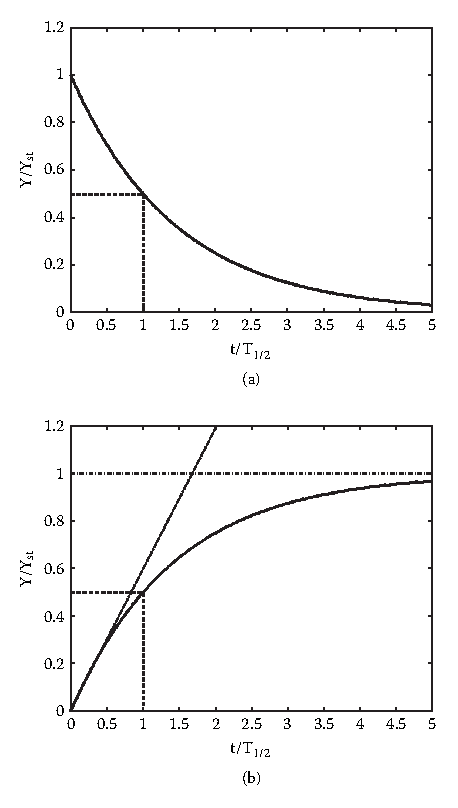
\includegraphics{Chapters/chapter1/figures/002x006.eps}
\caption[The bar charts depict the different risk contributions]{The bar charts depict the different risk contributions (top: 99\% quantile, bottom: 99.9\% quantile) of the business areas of a bank. The black bars
are based on a Var/Covar approach, the white ones correspond to shortfall risk.}
\end{figure}


\begin{exerciselist}

%%\textsc{\textbf{EXERCISES}}

\item \textit{A change in production rate}. A gene Y with simple regulation is produced at a constant rate $\beta 
_{1}$. The production rate suddenly shifts to a different rate $\beta 
_{2}$.

\item \textit{A change in production rate}. A gene Y with simple regulation is produced at a constant rate $\beta 
_{1}$. The production rate suddenly shifts to a different rate $\beta 
_{2}$.

\item \textit{A change in production rate}. A gene Y with simple regulation is produced at a constant rate $\beta 
_{1}$. The production rate suddenly shifts to a different rate $\beta 
_{2}$.

\item \textit{A change in production rate}. A gene Y with simple regulation is produced at a constant rate $\beta 
_{1}$. The production rate suddenly shifts to a different rate $\beta 
_{2}$.

\item \textit{A change in production rate}. A gene Y with simple regulation is produced at a constant rate $\beta 
_{1}$. The production rate suddenly shifts to a different rate $\beta 
_{2}$.

\item \textit{A change in production rate}. A gene Y with simple regulation is produced at a constant rate $\beta 
_{1}$. The production rate suddenly shifts to a different rate $\beta 
_{2}$.


\item \textit{A change in production rate}. A gene Y with simple regulation is produced at a constant rate $\beta 
_{1}$. The production rate suddenly shifts to a different rate $\beta 
_{2}$.

\item \textit{A change in production rate}. A gene Y with simple regulation is produced at a constant rate $\beta 
_{1}$. The production rate suddenly shifts to a different rate $\beta 
_{2}$.

\begin{enumerate}
\item Calculate and plot the gene product concentration Y(t).

\item What is the response time (time to reach halfway between the steady 
states)?
\end{enumerate}

\textit{Solution} (\textit{for part a})$:$

\begin{enumerate}
\item
 Let us mark the time when the shift occurs as t = 0. Before the shift, Y 
reaches steady state at a level Y(t = 0) = Y$_{st}=\beta _{1}$/$\alpha 
$. After the shift,
\begin{equation}
dY/dt = \beta _2 - \alpha \,Y
\end{equation}

The solution of such an equation is generally Y = C$_{1} \quad {\rm r}$ C$_{2}$ 
e$^{\mbox{--}\alpha } \quad ^{t}$, where the constants C$_{1}$ and C$_{2}$ need 
to be determined so that Y(t = 0) = $\beta _{1}$/$\alpha $, and Y at long 
times reaches its new steady state, $\beta _{2}$/$\alpha $. This yields 
the following sum of an exponential and a constant:

$Y(t) = \beta _2 \mbox{ / }\alpha + (\beta _1 \mbox{ / }\alpha - \beta _2 
\mbox{ / }a)e^{ - \alpha \,t}$(P2.2)

Take the derivative with respect to time, dY/dt, and verify that Equation 
P2.1 is fulfilled.
\end{enumerate}

\item \textit{mRNA dynamics}. In the main text, we considered the activation of transcription of a 
gene (mRNA production) and used a dynamical equation to describe the changes 
in the concentration of the gene product, the protein Y. In this equation, 
dY/dt = $\beta $ -- $\alpha $ Y, the parameter $\beta $ describes the rate 
of protein production. In reality, mRNA needs to be translated to form the 
protein, and mRNA itself is also degraded by specific enzymes.

\begin{enumerate}
\item Derive dynamical equations for the rate of change of mRNA and the rate of 
change of the protein product, assuming that mRNA is produced at rate $\beta 
_{m}$ and degraded at rate $\alpha _{m}$, and that each mRNA produces on 
average p protein molecules per unit time. The protein is degraded/diluted 
at rate $\alpha $.

\item Note that mRNA is often degraded at a much faster rate than the protein 
product $\alpha _{m}$ >> $\alpha $. Can this be used to form a 
quasi-steady-state assumption that mRNA levels are at steady state with 
respect to slower processes? What is the effective protein production rate 
$\beta $ in terms of $\beta _{m}$, $\alpha _{m}$, and p? What would be 
the response time if the mRNA lifetime were much longer than the protein 
lifetime?
\end{enumerate}

\textit{Solution:}

\begin{enumerate}
\item The dynamic equation for the concentration of mRNA of gene Y, Y$_{m}$, 
is:
\begin{equation}
dY_m \mbox{ / }dt = \beta _m - \alpha _m Y_m 
\end{equation}

The dynamical equation for the protein product is due to production of p 
copies per mRNA and degradation/dilution at rate $\alpha $:
\begin{eqnarray}
dY_m \mbox{ / }dt &=& \beta _m - \alpha _m Y_m \\
dY\mbox{ / }dt &=& p\,Y_m - \alpha \,Y
\end{eqnarray}
\item
 In the typical case that mRNA degradation is faster than the 
degradation/dilution of the protein product, we can assume that Y$_{m}$ 
reaches steady state quickly in comparison to the protein levels. The reason 
is that the typical time for the mRNA to reach steady state is the response 
time log(2)/$\alpha _{m}$, which is much shorter than the protein response 
time log(2)/$\alpha $ because $\alpha _{m}$ >> $\alpha $. The steady-state 
mRNA level is found by setting dY$_{m}$/dt = 0 in Equation P2.3, yielding



Using this for Y$_{m}$ in Equation P2.4 yields the following equation for 
the protein production rate:


In other words, the effective protein production rate, which is the first 
term on the right-hand side of the equation, is equal to the steady-state 
mRNA level times the number of proteins translated from each mRNA per unit 
time:
\begin{equation}
\beta = p\,\beta _m /\alpha_m
\end{equation}

\end{enumerate}

\item \textit{Time-dependent production and decay}. A gene Y with simple regulation has a time-dependent production rate 
$\beta $(t) and a time-dependent degradation rate $\alpha $(t). Solve for 
its concentration as a function of time.
\end{exerciselist}

\begin{VT1}

\VH{Think About It...}

Commonly thought of as the first modern computer, ENTAC was built in 1944. It took up more space than an 18-wheeler's
tractor trailer and weighed more than 17 Chevrolet Camaros. It consumed 140,000 watts of electricity while executing
up to 5,000 basic arithmetic operations per second. One of today's popular microprocessors, the 486, is built on a
tiny piece of silicon about the size of a dime.

\VT
With the continual expansion of capabilities, computing power will eventually exceed the capacity for human
comprehension or human control.

\VTA{The Information Revolution}{Business Week}
\end{VT1}



\begin{Glossary}
\item[360 Degree Review] Performance review that includes feedback from superiors, peers, subordinates, and clients.
\item[Abnormal Variation] Changes in process performance that cannot be accounted for by typical day-to-day variation. Also referred to as
non-random variation.
\item[Acceptable Quality Level (AQL)] The minimum number of parts that must comply with quality standards, usually stated as a percentage.
\item[Activity] The tasks performed to change inputs into outputs.
\item[Adaptable] An adaptable process is designed to maintain effectiveness and efficiency as requirements change. The process is
deemed adaptable when there is agreement among suppliers, owners, and customers that the process will meet
requirements throughout the strategic period.
\end{Glossary}


\begin{thefurtherreading}{99}

\bibitem{} Becskei, A. and Serrano, L. (2000). Engineering stability in gene networks 
by autoregulation. \textit{Nature, }405: 590--593.

\bibitem{} Rosenfeld, N., Elowitz, M.B., and Alon, U. (2002). Negative auto-regulation 
speeds the response time of transcription networks. \textit{J. Mol. Biol.}, 323: 785--793.

\bibitem{} Savageau, M.A. (1976). \textit{Biochemical Systems Analysis: A study of Function and Design in Molecular Biology. }Addison-Wesley. Chap. 16.

\bibitem{} Savageau, M.A. (1974). Comparison of classical and auto-genous systems of 
regulation in inducible operons. \textit{Nature}, 252: 546--549.
\end{thefurtherreading}